\section{Proposed Model}\label{prop}
We developed a new model for the force of infection in compartmental models
which aims to overcome the limitations of models \case{1-3}.
Below we describe the conceptual basis for the model, followed by the equations.
\subsection{Conceptual Development}\label{prop.cd}
Consider a population of 32 individuals in 16 partnerships with 25\% infection prevalence,
at the moment of one transmission (Figure~\ref{fig:tx.pairs}).
Initially, infection prevalence among partners
of susceptible $S$ (6/24) and infectious $I$ (2/8) individuals are equal.
Immediately after transmission, the prevalence
decreases to 5/23 among partners of $S$ but increases to 4/9 among partners of $I$, reducing incidence.
Next, two events are possible:
a) another transmission among the remaining discordant partnerships,
yielding 4/22 prevalence among partners of $S$ and 6/10 among partners of $I$,
further reducing incidence; or
b) the partnership from the first transmission ends
and both individuals form new partnerships at random,
yielding prevalence 9/32 among partners of both $S$ and $I$ (on average), increasing incidence.
Effectively, models \case{1-3} all assume that (b) occurs first,
but this assumption may be invalid, especially for long-duration partnerships.
Other partnerships may begin/end too before (a) or (b),
but the proportions of discordant partnerships would remain unchanged, on average.
\begin{figure}[h]
  \begin{subfigure}{\textwidth}
    % TODO: draw grey box here too? gets confusing after transmission as we need fractions
    \centerline{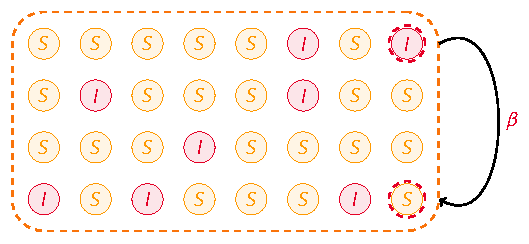
\includegraphics[scale=1]{tx.freq}}
    \caption{Frequentist approximation}
    \label{fig:tx.freq}
  \end{subfigure}
  \begin{subfigure}{\textwidth}
    \centerline{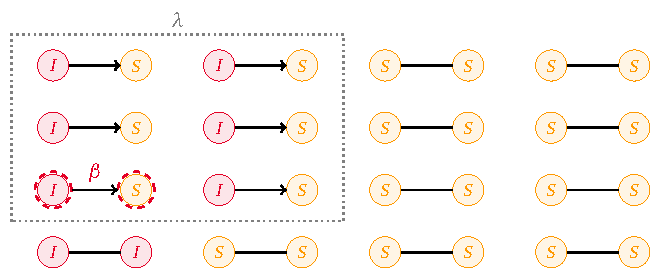
\includegraphics[scale=1]{tx.pairs}}
    \caption{Pair-wise reality}
    \label{fig:tx.pairs}
  \end{subfigure}
  \caption{Illustration of 32 individuals in a population with 25\% infection prevalence,
    at the moment of one transmission ($\beta$)}
  \label{fig:tx}
  \floatfoot
  Notation. $S$: susceptible; $I$: infectious; $\beta$: transmission event.
\end{figure}
\par
This scenario highlights how any partnership where transmission has occurred
should be ``removed'' from the force of infection.
% TODO: more discussion of pair-based models here? Or elsewhere...
In a compartmental (non-pair-based) model,
these partnerships can be tracked as proportions of individuals:
namely, all recently infected individuals \emph{and} all recently transmitting individuals.
If individuals have multiple concurrent partnerships ($C_{i} > 1$),
then these individuals should not be removed entirely,
but their effective numbers of partners should be reduced by 1.
If multiple types of partners are considered,
then only the type involved in transmission should be reduced.
This adjustment can then be applied until the individuals change partners
--- an expected period of $\delta_k$.
However, during this period, these individuals should be modelled
to progress as usual through different stages of infection, aging, etc.
\par
Using this conceptual basis,
we propose a new stratification of modelled population, denoted $\k$.
The stratum $\k = 0$ corresponds to no recent transmission, or all ``new'' partners.
Other strata $\k > 0$ correspond to recent transmission via (to or from) partnership type $k$.
Figure~\ref{fig:model.hk} illustrates the new stratification
for an system with 5 modelled infection stages.
Following infection, all individuals enter a stratum $\k > 0$
corresponding to the partnership type $k$ by which they were infected.
Thus, the rate of entry (from $S_i$) is $\lambda_{ik}$.
Individuals may then transition from $\k > 0$ to $\k = 0$
upon forming a new partnership, at a rate $\delta_k^{-1}$.
Finally, individuals may re-enter any stratum $\k > 0$
if they transmit infection via partnership type $k$.
We denote the corresponding rate as $\lambda'_{ik}$,
representing the per-person rate of \emph{transmission},
not \emph{acquisition} as in $\lambda_{ik}$.
This rate $\lambda'_{ik}$ is not usually defined,
but we develop the equations to do so below.
\begin{figure}
  \centerline{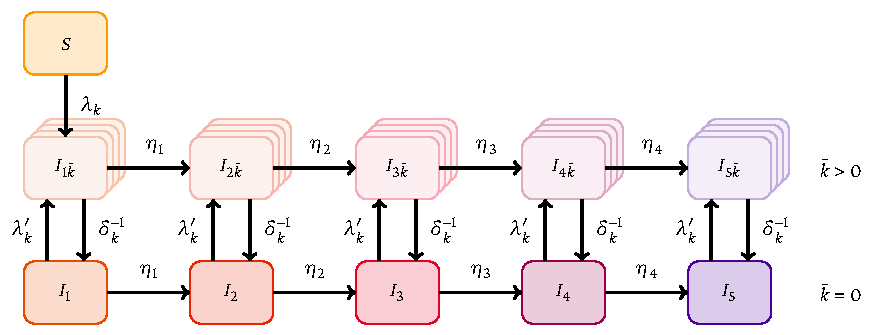
\includegraphics[scale=.95]{model.hiv.fpe}}
  \caption{Illustration of a new stratification $\k$ to track
    proportions of individuals in partnerships where transmission has already occurred.}
  \label{fig:model.hk}
  \floatfoot
  Notation.
  $S$: susceptible;
  $I_h$: infectious in stage $h$;
  $k$: partnership type;
  $\k$: new stratification;
  $\lambda$: force of infection to susceptible;
  $\lambda'$: force of infection from infectious;
  $\eta$: rate of progression between infection stages;
  $\delta$: duration of partnership.
\end{figure}
\subsection{Equations}\label{prop.eq}
Since partnership duration is now considered separately,
we start from the pure rate model \case{3}.
We adapt \eqref{eq:foi.3} to:
integrate the changes to mixing due to changes in numbers of partners available; and
track the rate of transmission \emph{from} risk groups $j$ and infection stages $h$.
\par
We begin by defining $M_{ijk}$ as the absolute (not per-person) number of
type-$k$ partnerships between group~$i$ and group~$j$.
We assume that $M_{ijk}$ can be defined by an arbitrary function $f$,
with inputs $M_{ik}$, $M_{jk}$, and some parameter(s) $\theta_{ijk}$ specifying mixing patterns:
\begin{equation}
  M_{ijk} = f(M_{ik}, M_{jk}, \theta_{ijk})
\end{equation}
We define $M_{ik}$ (and likewise $M_{jk}$) as the total numbers of
type-$k$ partnerships ``offered'' by group $i$,
across both susceptible and infected individuals in each infection stage $h$:
\begin{equation}
  M_{ik} = M_{S,ik} + \sum_h M_{I,ihk}
\end{equation}
We define $M_{S,ik}$ and $M_{I,ihk}$ as follows:
\begin{subequations}\label{eq:M.SI}
  \begin{alignat}{1}
    M_{S,ik}  &= \label{eq:M.S}
    S_{i} C_{ik} \\
    M_{I,ihk} &= \label{eq:M.I}
    I_{ih,\,\k=k} (C_{ik}-1) + \textstyle\sum_{\k\ne k} I_{ih,\k} C_{ik}
  \end{alignat}
\end{subequations}
The definition \eqref{eq:M.S} is hopefully familiar,
while \eqref{eq:M.I} can be described as the sum of partnerships ``offered'' across states $\k$,
where the partnership numbers $C_{ik}$ of infected individuals in state $\k=k$ are reduced by 1.
\par
Next, we define the absolute (not per-person) rate of transmission
from group $j$ and infection stage $h$ to group $i$ via type-$k$ partnerships as:
\begin{equation}
  \Lambda_{ijhk} = F_k \beta_{hk} M_{ijk} \frac{M_{S,ik}}{M_{ik}} \frac{M_{I,jhk}}{M_{jk}}
\end{equation}
where the two fractions represent the proportions of all partnerships ($M_{ijk}$)
formed by susceptible individuals in group $i$ ($M_{S,ik}$)
with infectious individuals in group $j$ and infection stage $h$ ($M_{I,jhk}$).
Finally, we define the per-person transmission rates
to $i$ and from $jh$ as follows:
\begin{equation}\label{eq:foi.i}
  \lambda_{ik} = \sum_{jh} \frac{\Lambda_{ijhk}(t)}{S_{i}}
\end{equation}
\begin{equation}\label{eq:foi.jh}
  \lambda'_{jhk} = \sum_{i} \frac{\Lambda_{ijhk}(t)}{I_{jh}}
\end{equation}
For the purposes of solving the model,
we can even skip division by $S_i$ and $I_{jh}$ in \eqref{eq:foi.i}~and~\eqref{eq:foi.jh},
since $\lambda'_{ik}$ and $\lambda'_{jhk}$ are immediately multiplied by $S_i$ and $I_{jh}$,
respectively, in the system of differential equations.
\subsection{Comment}
In the proposed approach, we do not explicitly model the proportion of infected individuals
who recently transmitted or acquired infection via two \emph{different} partnership types,
(or two partnerships of the same type).
If we did, the required size of the new dimension $\k$ would be $2^{K}$, not $K+1$.
However, under frequentist assumptions, we can equivalently model
two transmissions by one individual as one transmission each by two individuals,
and thus allocate two proportions of $I_{jh\k=0}$ to $I_{jh\k=k_1}$ and $I_{jh\k=k_2}$ (one each),
instead of just one proportion to $I_{jh\k={(k_1k_2)}}$.
\par
In fact, $I_{jh\k=0}$ can be \emph{negative},
because the dimension $\k$ is only relevant to \eqref{eq:M.I},
and in all other contexts and equations,
we first sum $I_{jh\k}$ across $\k$ to yield $I_{hj}$, which should be positive.
Moreover, we can also have $I_{jh\k} > I_{jh}$, provided that $I_{jh\k} \le I_{jh} C_{jk}$,
reflecting the situation when more than 100\% of $I_{jh}$
have recently transmitted or acquired infection via at least one type-$k$ partnership.
This situation can only arise in the context of concurrent partnerships, $C_{jk} > 1$.
In this case $I_{jh\k=0}$ \emph{must} be negative,
but it can be shown that \eqref{eq:M.I} still yields the correct value of $M_{I,ihk}$.
With this perspective, the constraint $I_{jh\k} \le I_{jh} C_{jk}$ may be intuitive,
and it should be possible to guarantee for small enough timesteps,
because $M_{I,ihk}$ approaches zero as $I_{jh\k}$ approaches $I_{jh} C_{jk}$
--- i.e. all partnerships become concordant.
% TODO: discuss the possibility of being in multiple seroconcordant partnerships following transmission
% slightly more complicated modelling of transitions within "k" dimension,
% with main risk if we don't being: run out of people in k=0 (fully discordant)